\documentclass[a4paper]{article}
\usepackage{forest}
\usepackage{float}
\usepackage{makecell}
\usepackage{geometry}
\usepackage{listings}
\usepackage{hyperref}
\usepackage{graphicx}
\usepackage{ragged2e}
\usepackage{color}
\usepackage{xepersian}
\usepackage{subfiles}
\settextfont[Scale=1]{XB Roya}

\title{زبان‌های \lr{Orchestration} و \lr{Choreography}}
\author{علیرضا سلطانی نشان}

\begin{document}
\maketitle

\section{\lr{Service Choreography}}

در این مدل از مدیریت سرویس‌ها، هر سرور از وظیفه خود آگاه است و براساس قوانین و
ارتباطاتی که دارد به صورت مستقیم به سرور و سرویس‌های دیگر متصل است و با یکدیگر
کار می‌کنند. دقیقاً همانند اعضای بدن که هر کدام وظیفه مشخصی دارند ولی با همکاری
با یکدیگر می‌توانند به یک هدف مشترک برسند و در صورت عدم حضور صحیح یکی از اعضا
عملکرد تمام اعضا تحت تاثیر قرار می‌گیرد. در این مدل هیچ \lr{Central control}
حضور ندارد و سرویس‌ها براساس رخداد‌ها یا \lr{Event} با یکدیگر تعامل دارند
\cite{cvom}. از مزیت استفاده از این مدل می‌توان به موارد زیر اشاره کرد:

\begin{itemize}
    \item عدم کنترل متمرکز: این کار باعث می‌شود تا مقیاس‌پذیری و تحمل خطا افزایش
    پیدا‌ کند چرا که هیچ گونه \lr{Single point of failure} در آن وجود ندارد که
    با خراب شدن سیستم مرکزی عملکرد کل سیستم مختل شود و سیستم در حالت بلاتکلیف
    قرار گیرد.
    \item این روش برای معماری‌های مبتنی بر رخداد بهطور مناسب کار می‌کند. این مدل
    کاملاً برای سیستم‌هایی که نیاز به پردازش \lr{Real-time} دارند مناسب است.
\end{itemize}

معایب استفاده از این مدل عبارت‌اند از:

\begin{itemize}
    \item پیچیدگی در مدیریت، زمانی که اعضای حاضر در سیستم افزایش یابد مدیریت
    تعاملات سیستم‌ها با یکدیگر دشوارتر می‌شود.
    \item این مدل همواره با چالش‌های پایش و \lr{debugging} رو به رو است.
\end{itemize}

\begin{figure}[H]
    \centering
    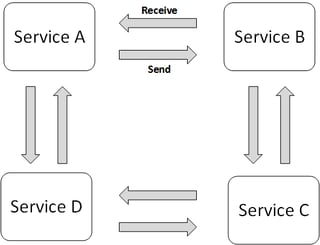
\includegraphics[width=0.3\textwidth]{choreography.jpeg}
    \caption{عدم وجود سرویس مرکزی و تعامل سرویس‌ها به صورت \lr{Peer to peer}
    \cite{stackoverflow}}
    \label{fig:atmDiagram}
\end{figure}

\subsection*{مثال کاربردی}

در فروشگاه‌های هوشمند که تمام سیستم‌ها به صورت مستقل وظایف مشخصی دارند. هر
سرویسی به سرویس دیگر به صورت مرحله‌ای نیازمند است. تصور کنید که مشتری محصولی را
انتخاب کرده است، سفارش محصول به سمت سرویس انبارداری منتقل می‌شود تا مشخص شود از
این محصول به تعداد درخواست شده موجودی کالا بررسی شود. بعد از بررسی سرویس
انبارداری به سرویس بررسی سبد محصولات هدایت می‌شود تا خرید و سفارش خود را نهایی
کند. سپس بعد از نهایی سازی سفارشات به سرویس پرداخت منتقل می‌شود و در صورتی که
پرداخت موفقیت‌آمیزی داشته باشد سرویس پیک برای ارسال محصول به مشتری صدا زده
می‌شود. این سرویس‌ها در سیستم فروشگاه هوشمند تماماً براساس رخدادهایی کار می‌کنند
که توسط سرویس‌های پیشین صدا زده می‌شوند.

\section{Service Orchestration}

در این مدل یک \lr{Central orchestrator} وجود دارد که وظیفه مدیریت تعاملات بین
سرویس‌ها را به طور مرکزی دارد. یعنی اگر سیستم مرکزی نباشد هیچ تسکی بین سرویس‌ها
توزیع نمی‌شود و سرویس‌ها با هدر رفت منابع رو به رو خواهند بود \cite{cvom}. از
مزیت این مدل تعامل می‌توان به موارد زیر اشاره کرد:

\begin{itemize}
    \item کنترل مرکزی: که دائما ویژگی \lr{Single point of control} را ارائه
    می‌دهد پیاده‌سازی راحت‌تری را نسبت به مدل تعامل قبلی ارائه می‌دهد.
    \item کنترل خطای بهتر: یک \lr{Ochestrator} می‌تواند به صورت بهینه‌تری
    \lr{Retry}ها، \lr{Rollback}ها و جریان‌های جایگزین را مدیریت کند چرا که از
    بالا دستورات به صورت سلسله مراتبی و درختی به نود‌های (سرویس‌های) پایینی
    منتقل می‌شود و می‌توان وضعیت هر کدام از سرویس‌ها را از بالا پایش و
    \lr{Debug} کرد.
    \item مدیریت بهتر گزارش‌ها: در مدل تعامل \lr{Orchestration} لاگ‌اندازی و
    پایش تمام فرایند‌ها بهتر از مدل \lr{Choreography} می‌باشد و می‌توان از طریق
    این فرایند وضعیت بعدی سیستم را پیش‌بینی کرد.
\end{itemize}

مهم‌ترین عیب این مدل تعامل وجود سیستم مرکزی برای مدیریت سرویس‌ها می‌باشد چرا که
ممکن است با هر \lr{Single point of failure} کل سیستم \lr{Down} شود زیرا
سرویس‌های زیرین تماماً تحت تاثیر دستورات سیستم مرکزی هستند و اینکار باعث می‌شود
سرویس‌ها تسک‌های خود را دریافت نکنند و عملاً فرایندی شروع نشود. یا اگر در حین
کار سیستم مرکزی از کار افتد سرویس‌های زیرین در وضعیت بلاتکلیف باقی می‌مانند و
نمی‌توانند ادامه فرایند را پیش روند.

\begin{figure}[H]
    \centering
    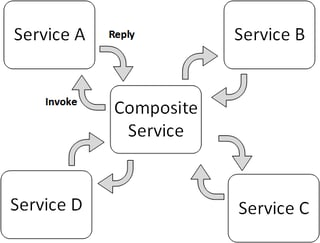
\includegraphics[width=0.3\textwidth]{orchestration.jpeg}
    \caption{تعامل سیستم‌ها ابتدا توسط سیستم مرکزی اتفاق می‌افتد زیرا از سیستم
    مرکزی تسک خود را دریافت می‌کنند \cite{stackoverflow}.}
    \label{fig:atmDiagram}
\end{figure}

همانطور که آقای \lr{Karel Husa} \cite{karelhusaOpinion} در استک اورفلو گفته است،
ما نیازی به تفاوت قائل شدن بین دو مدل تعامل و ارتباطات \lr{Orchestration} و
\lr{Choreography} نداریم، نیازمندی اصلی ما تمرکز روی منطق کسب و کار سیستم است.
به عبارت دیگر، انتخاب میان این دو مدل به نوع مسئله و نیازمندی‌های آن بستگی دارد
نه به یک تعریف تئوریک. مدل \lr{Orchestration} به دلیل ماهیت تمرکز، در دنیای
\lr{IT} کاربرد بیشتری دارد، در حالی که \lr{Choreography} معمولاً به عنوان یک
موضوع تحقیقاتی باقی می‌ماند اما ممکن است به صورت غیرآگاهانه در برخی سیستم‌ها
مورد استفاده قرار گیرد.

چرا \lr{Choreography} از نظر توسعه‌دهندگان تنها در آکادمیک باقی می‌ماند؟

دلیل اصلی آن این است که برای ایجاد هماهنگی در سیستم‌هایی که به صورت غیرمتمرکز
هستند تلاش بسیار زیادی باید صورت گیرد تا به نتیجه مورد نظر برسد و در بسیاری از
سرویس‌های امروزی، ما بدون اینکه بدانیم مدل تعامل \lr{Choreogprahy} چه چیزی
می‌باشد به صورت غیرمتمرکز سرویس‌های خود را با یکدیگر هماهنگ‌سازی می‌کنیم.

\section{\lr{Architecture Definition Languages}}

\lr{ADL}ها نقش اساسی در طراحی و مشخص کردن رفتار سیستم‌های توزیع شده دارند، علل
خصوص در مدل‌های \lr{Orchestration} و \lr{Choreography}:

\subsection{زبان‌های \lr{Orchestration}}

\begin{enumerate}
    \item زبان \lr{WS-BPEL} یا \lr{Web Services Business Process Execution
    Language}: یک زبان رسمی برای مشخص کردن المان‌ها و روابط آن‌ها در سرویس‌های
    وب در مدل \lr{Orchestration} بکار می‌رود. در حین پیاده‌سازی ممکن است با
    پیچیدگی‌هایی رو به رو شویم.
    \item \lr{UML} یا \lr{Unified Modeling Language}: با استفاده از این زبان
    می‌توان برای مدل‌های \lr{Orchestration} با استفاده از \lr{Activity diagram}
    روابط بین المان‌ها را مشخص کرد.
\end{enumerate}

\subsection{زبان‌های \lr{Choreography}}

\begin{enumerate}
    \item \lr{WS-CDL} یا \lr{Web Services Choreography Description Language}: به
    صورت مشخص روی تعریف مدل \lr{Choreography} وب سرویس‌ها مورد استفاده قرار
    می‌گیرد.
    \item \lr{Pi-Calculus}: از یک زبان ریاضی برای تعریف سیستم‌های موبایل و روابط
    داخلی آن‌ها استفاده می‌کند. یک زبان رسمی برای استدلال در مورد سیستم‌های
    همروند ارائه می‌دهد.
\end{enumerate}

\bibliographystyle{unsrt-fa}
\bibliography{interoperatibility_refs.bib}
\end{document}
